\documentclass[11pt]{article}
\usepackage[margin=1in]{geometry}
\usepackage[nolist]{acronym}
\usepackage{array}
\usepackage{booktabs}
\usepackage{tabularx}
\usepackage{longtable}
\usepackage{graphicx}
\usepackage{tikz}
\usetikzlibrary{positioning,calc,arrows.meta}

\acrodef{gwg}{gestational weight gain}
\acrodef{bmi}{body mass index}

\begin{document}

\section{Protopersona Profiles}
\label{app:protopersona-profiles}

Table~\ref{tab:protopersona_comparison} summarises the main characteristics, needs, and design implications associated with the three protopersonas developed during the expert-informed user modelling phase.

\begin{table*}[ht]
\centering
\caption{Comparative Overview of the Three MATER Protopersonas}
\label{tab:protopersona_comparison}
\begin{tabular}{p{3cm}p{3.8cm}p{3.8cm}p{3.8cm}}
\hline
\textbf{Dimension} & 
\textbf{Giulia Bianchi} \newline \emph{Informed but Overwhelmed} &
\textbf{Martina Rossi} \newline \emph{Time-Constrained Multitasker} &
\textbf{Elena Verdi} \newline \emph{Nutritionally Conscious User} \\
\hline

\textbf{Profile} &
Primiparous woman (30-35), highly educated, proactive in health information seeking. &
Pregnant woman (30-40), often multiparous, balancing work and family responsibilities. &
Pregnant woman (30-35) following a vegetarian or vegan diet with strong nutritional awareness. \\

\textbf{Primary Needs} &
Evidence-based information, clear explanation of gestational weight gain, trimester-specific guidance, reassurance on physiological changes. &
Concise and actionable guidance, quick monitoring tools, practical meal solutions. &
Diet-specific recommendations, reassurance on nutrient adequacy, detailed explanations on supplementation and food safety. \\

\textbf{Main Barriers / Frustrations} &
Conflicting online information, difficulty identifying reliable sources, anxiety about weight monitoring. &
Time constraints, difficulty maintaining structured meal planning, excessive data-entry burden. &
Generic dietary advice not adapted to plant-based diets, insufficient personalisation. \\

\textbf{Behavioural Traits} &
High digital engagement, frequent consultation of apps and professionals, strong adherence to validated recommendations. &
Goal-oriented interaction, sporadic tracking, efficiency-driven behaviours. &
Highly proactive, careful nutrient monitoring, strong interest in detailed nutritional information. \\

\textbf{Design Implications for MATER} &
Transparent sources, myth-debunking sections, structured educational pathways, reassuring weight monitoring feedback. &
Streamlined interface, simplified tracking, quick food logging, visual weight trends, ready-to-use meal templates. &
Diet-specific pathways (omnivorous/vegetarian/vegan), micronutrient indicators, advanced educational modules. \\

\hline
\end{tabular}
\end{table*}

\textbf{Giulia Bianchi - The ``Informed but Overwhelmed'' First-Time Mother}

Giulia Bianchi represents a primiparous woman aged 30-35 years, with high educational attainment (university degree or postgraduate education) and strong autonomy in health management. She demonstrates high engagement in information-seeking behaviours and actively consults healthcare professionals, institutional sources, and pregnancy-tracking applications.

Compared to multiparous women, she shows greater attentiveness to nutritional management and a stronger need for validated information.

\textit{Primary Needs:}
Evidence-based and clearly structured information; explicit explanation of gestational weight gain recommendations; trimester-specific guidance; reassurance regarding physiological weight changes.

\textit{Frustrations:}
Conflicting online information; difficulty identifying scientifically validated sources; anxiety related to gestational weight monitoring; confusion about permitted and restricted foods.

\textit{ Behavioural Traits:}
High digital engagement; continuous use of weight and trimester-tracking apps; proactive consultation of professionals to confirm online information; strong adherence to recommendations once clearly explained.

\textit{Design Implications for MATER:}
Clear explanation of gestational weight gain targets contextualised to pre-pregnancy body mass index; explicit source transparency; structured educational pathways; reassuring feedback mechanisms in weight monitoring; integrated myth-debunking sections to counter misinformation.

\vspace{0.5em}

\textbf{Martina Rossi - The ``Time-Constrained Multitasker''}

Martina Rossi represents a pregnant woman aged 30-40 years, often multiparous, balancing professional responsibilities and family context. Time constraints may act as a barrier to strict adherence to dietary recommendations, particularly in meal preparation and planning.

\textit{Primary Needs:}
Concise and actionable dietary guidance; practical meal solutions; minimal time investment for monitoring; quick visual feedback.

\textit{Frustrations:}
Time-intensive meal preparation; difficulty maintaining structured eating routines; excessive data-entry burden; complex or overly theoretical explanations.

\textit{ Behavioural Traits:}
Continuous weight monitoring; sporadic dietary tracking; goal-oriented and efficiency-driven interactions; greater vulnerability to contextual (family/work-related) barriers.

\textit{Design Implications for MATER:}
Streamlined interface design; simplified tracking systems; quick-log food options; visual weight trend graphs; ready-to-use weekly meal templates; adaptive reminders compatible with busy schedules.
\vspace{0.5em}

\textbf{Elena Verdi - The ``Nutritionally Conscious and Proactive User''}

Elena Verdi represents a pregnant woman (30-35 years) following a vegetarian or vegan dietary pattern. She demonstrates high nutritional awareness and strong proactivity in ensuring adequacy of nutrient intake and food safety during pregnancy.

\textit{Primary Needs:}
 Personalised dietary guidance tailored to specific eating patterns; reassurance about nutrient adequacy; detailed but clear explanations regarding supplementation and food safety.

\textit{Frustrations:}
Generic dietary advice not adapted to plant-based diets; insufficient personalisation; lack of professional acknowledgment of her prior knowledge.

\textit{ Behavioural Traits:}
High adherence to recommendations; careful attention to nutrient adequacy; proactive questioning during consultations; interest in detailed nutritional breakdowns.

\textit{Design Implications for MATER:}
Diet-specific pathways (omnivorous, vegetarian, vegan); micronutrient adequacy indicators; tailored educational modules; optional advanced-content sections for highly engaged users.


\begin{figure*}[!t]
\centering
\resizebox{\textwidth}{!}{%
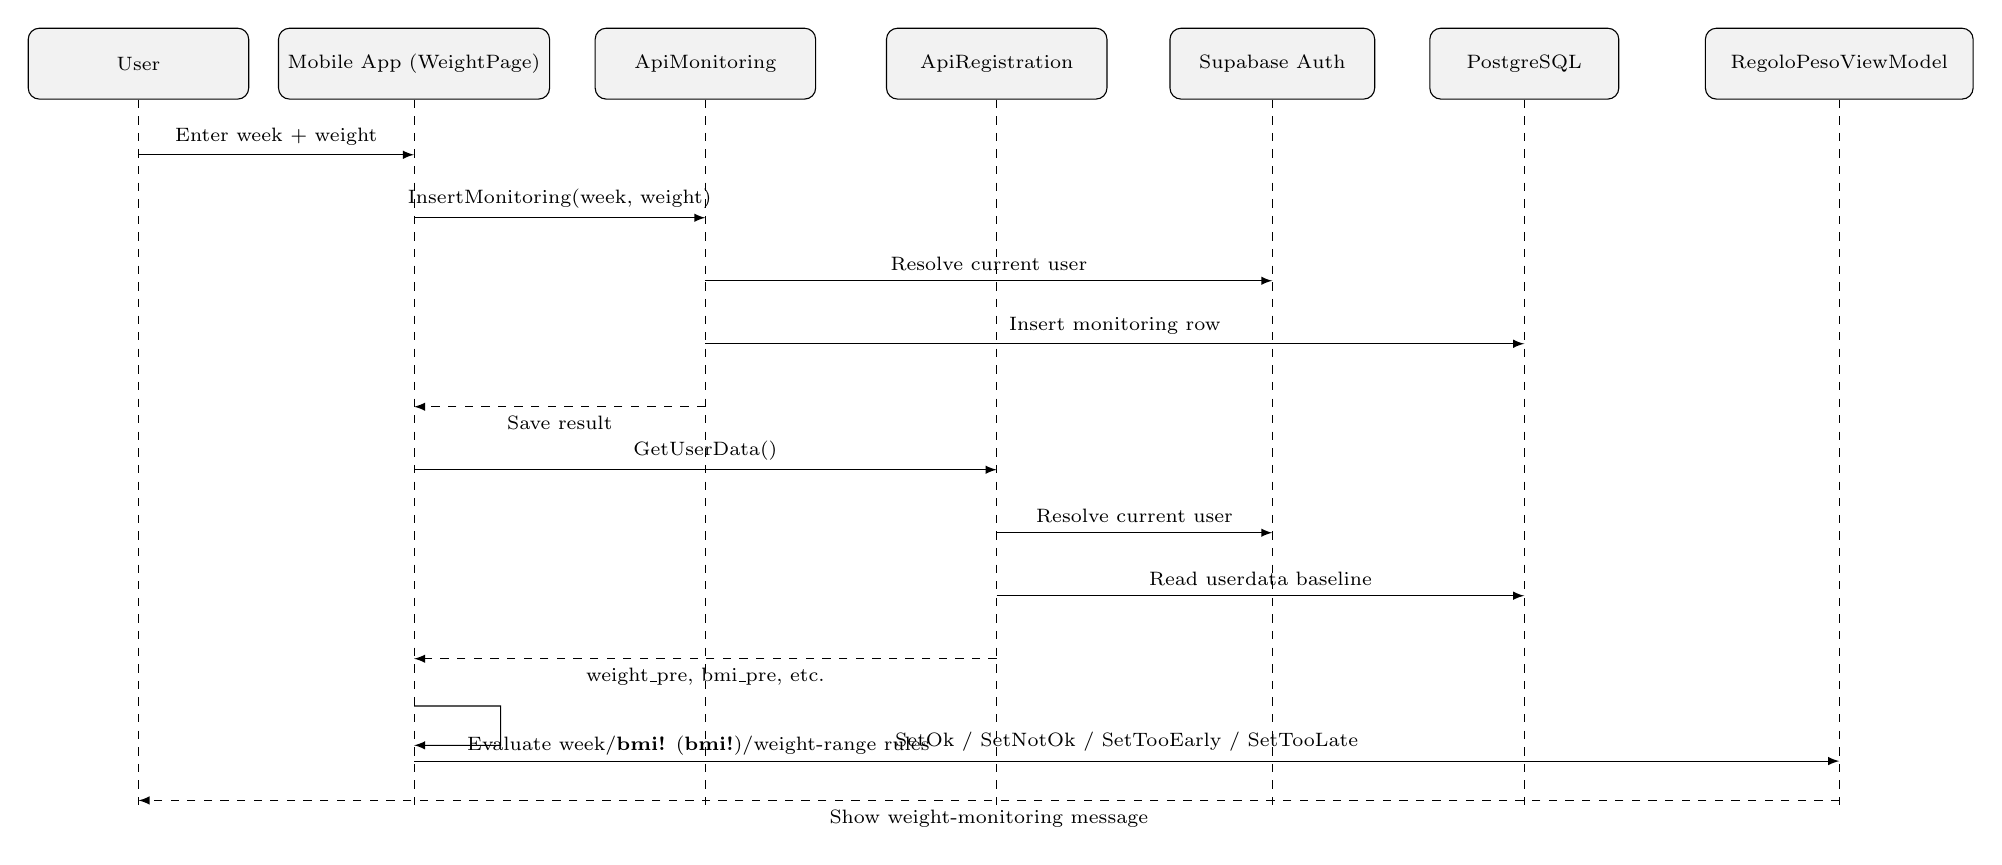
\begin{tikzpicture}[>=latex,font=\scriptsize]
  \node[draw,rounded corners,fill=gray!10,minimum width=2.8cm,minimum height=0.9cm] (u) at (0,0) {User};
  \node[draw,rounded corners,fill=gray!10,minimum width=3.2cm,minimum height=0.9cm] (app) at (3.5,0) {Mobile App (WeightPage)};
  \node[draw,rounded corners,fill=gray!10,minimum width=2.8cm,minimum height=0.9cm] (apimon) at (7.2,0) {ApiMonitoring};
  \node[draw,rounded corners,fill=gray!10,minimum width=2.8cm,minimum height=0.9cm] (apireg) at (10.9,0) {ApiRegistration};
  \node[draw,rounded corners,fill=gray!10,minimum width=2.6cm,minimum height=0.9cm] (auth) at (14.4,0) {Supabase Auth};
  \node[draw,rounded corners,fill=gray!10,minimum width=2.4cm,minimum height=0.9cm] (db) at (17.6,0) {PostgreSQL};
  \node[draw,rounded corners,fill=gray!10,minimum width=3.4cm,minimum height=0.9cm] (fb) at (21.6,0) {RegoloPesoViewModel};

  \foreach \n in {u,app,apimon,apireg,auth,db,fb} {
    \draw[dashed] (\n.south) -- ([yshift=-9.0cm]\n.south);
  }

  \draw[->] ([yshift=-0.7cm]u.south) -- node[above,sloped]{Enter week + weight} ([yshift=-0.7cm]app.south);
  \draw[->] ([yshift=-1.5cm]app.south) -- node[above,sloped]{InsertMonitoring(week, weight)} ([yshift=-1.5cm]apimon.south);
  \draw[->] ([yshift=-2.3cm]apimon.south) -- node[above,sloped]{Resolve current user} ([yshift=-2.3cm]auth.south);
  \draw[->] ([yshift=-3.1cm]apimon.south) -- node[above,sloped]{Insert monitoring row} ([yshift=-3.1cm]db.south);
  \draw[->,dashed] ([yshift=-3.9cm]apimon.south) -- node[below,sloped]{Save result} ([yshift=-3.9cm]app.south);

  \draw[->] ([yshift=-4.7cm]app.south) -- node[above,sloped]{GetUserData()} ([yshift=-4.7cm]apireg.south);
  \draw[->] ([yshift=-5.5cm]apireg.south) -- node[above,sloped]{Resolve current user} ([yshift=-5.5cm]auth.south);
  \draw[->] ([yshift=-6.3cm]apireg.south) -- node[above,sloped]{Read userdata baseline} ([yshift=-6.3cm]db.south);
  \draw[->,dashed] ([yshift=-7.1cm]apireg.south) -- node[below,sloped]{weight\_pre, bmi\_pre, etc.} ([yshift=-7.1cm]app.south);

  \draw[->] ([yshift=-7.7cm]app.south) -- ++(1.1,0) -- ++(0,-0.5) -- node[right]{Evaluate week/\ac{bmi}/weight-range rules} ([yshift=-8.2cm]app.south);
  \draw[->] ([yshift=-8.4cm]app.south) -- node[above,sloped]{SetOk / SetNotOk / SetTooEarly / SetTooLate} ([yshift=-8.4cm]fb.south);
  \draw[->,dashed] ([yshift=-8.9cm]fb.south) -- node[below,sloped]{Show weight-monitoring message} ([yshift=-8.9cm]u.south);
\end{tikzpicture}%
}
\caption{Weight-monitoring workflow across mobile app, API services, authentication, and database layers.}
\label{fig:weight-sequence}
\end{figure*}

\section{Data Model and System Architecture}
\begin{figure*}[!t]
\centering
\resizebox{\textwidth}{!}{%
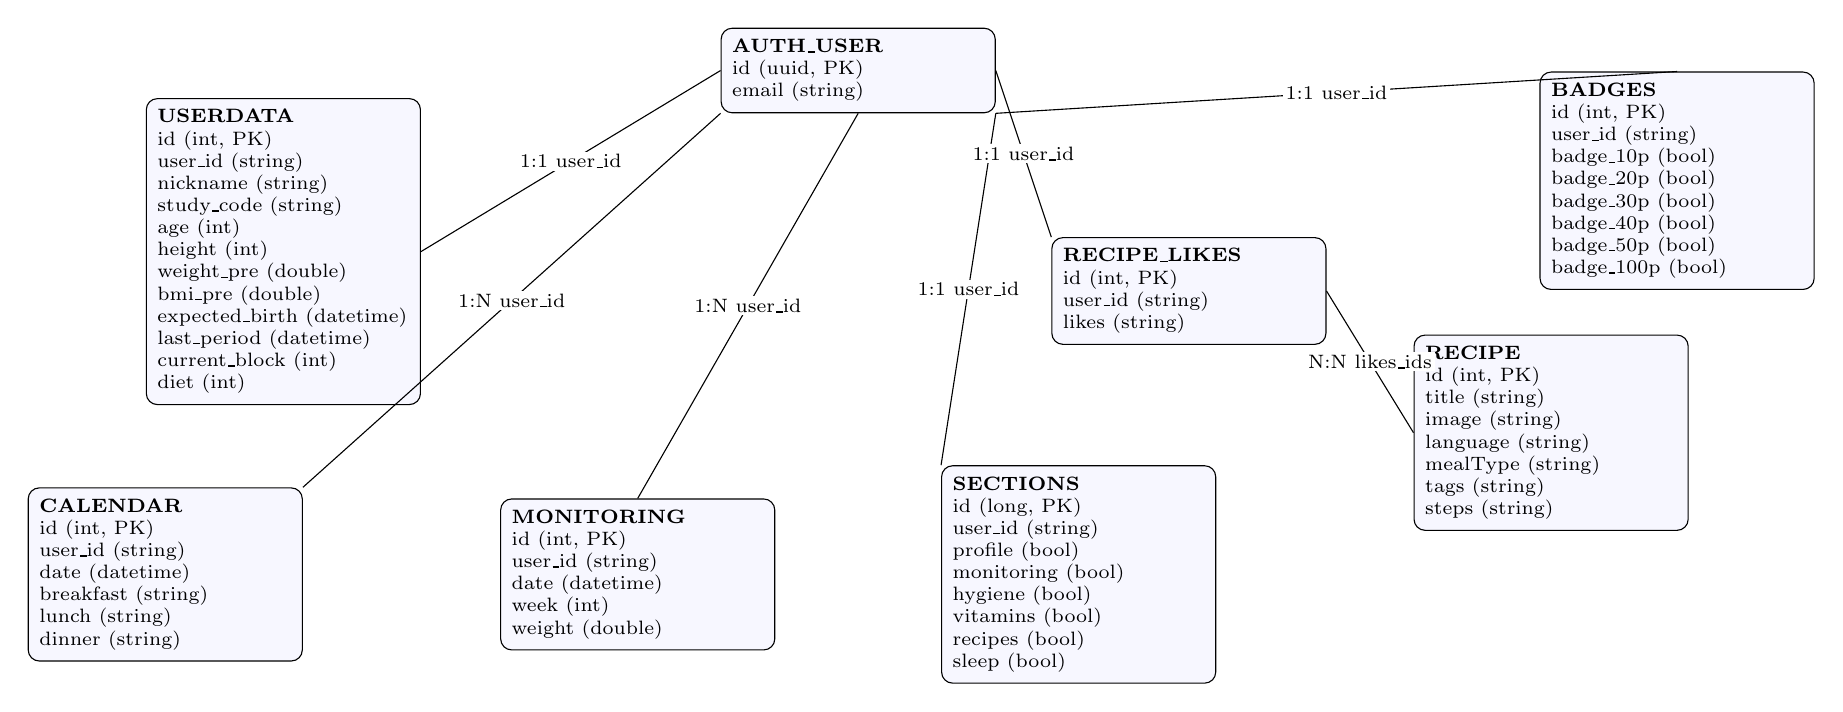
\begin{tikzpicture}[font=\scriptsize,>=latex]
  \tikzset{
    entity/.style={
      draw,
      rounded corners,
      fill=blue!3,
      align=left,
      inner sep=4pt,
      text width=3.2cm
    }
  }

  \node[entity] (auth) at (0,0) {\textbf{AUTH\_USER}\\id (uuid, PK)\\email (string)};

\node[entity] (userdata) at (-7.3,-2.3) {\textbf{USERDATA}\\id (int, PK)\\user\_id (string)\\nickname (string)\\study\_code (string)\\age (int)\\height (int)\\weight\_pre (double)\\bmi\_pre (double)\\expected\_birth (datetime)\\last\_period (datetime)\\current\_block (int)\\diet (int)};

  \node[entity] (calendar) at (-8.8,-6.4) {\textbf{CALENDAR}\\id (int, PK)\\user\_id (string)\\date (datetime)\\breakfast (string)\\lunch (string)\\dinner (string)};

  \node[entity] (monitoring) at (-2.8,-6.4) {\textbf{MONITORING}\\id (int, PK)\\user\_id (string)\\date (datetime)\\week (int)\\weight (double)};

  \node[entity] (sections) at (2.8,-6.4) {\textbf{SECTIONS}\\id (long, PK)\\user\_id (string)\\profile (bool)\\monitoring (bool)\\hygiene (bool)\\vitamins (bool)\\recipes (bool)\\sleep (bool)};

  \node[entity] (badges) at (10.4,-1.4) {\textbf{BADGES}\\id (int, PK)\\user\_id (string)\\badge\_10p (bool)\\badge\_20p (bool)\\badge\_30p (bool)\\badge\_40p (bool)\\badge\_50p (bool)\\badge\_100p (bool)};

  \node[entity] (recipeLikes) at (4.2,-2.8) {\textbf{RECIPE\_LIKES}\\id (int, PK)\\user\_id (string)\\likes (string)};

  \node[entity] (recipe) at (8.8,-4.6) {\textbf{RECIPE}\\id (int, PK)\\title (string)\\image (string)\\language (string)\\mealType (string)\\tags (string)\\steps (string)};

  \draw[-] (auth.west) -- node[midway,fill=white,inner sep=1pt]{1:1 user\_id} (userdata.east);
  \draw[-] (auth.south west) -- node[midway,fill=white,inner sep=1pt]{1:N user\_id} (calendar.north east);
  \draw[-] (auth.south) -- node[midway,fill=white,inner sep=1pt]{1:N user\_id} (monitoring.north);
  \draw[-] (auth.south east) -- node[midway,fill=white,inner sep=1pt]{1:1 user\_id} (sections.north west);
  \draw[-] (auth.south east) -- node[midway,fill=white,inner sep=1pt]{1:1 user\_id} (badges.north);
  \draw[-] (auth.east) -- node[midway,fill=white,inner sep=1pt]{1:1 user\_id} (recipeLikes.north west);
  \draw[-] (recipeLikes.east) -- node[midway,fill=white,inner sep=1pt]{N:N likes\_ids} (recipe.west);
\end{tikzpicture}%
}
\caption{Logical data model and key relationships used by MATER.}
\label{fig:data-er}
\end{figure*}

\end{document}
